\documentclass{article}


\usepackage{arxiv}

\usepackage[utf8]{inputenc} % allow utf-8 input
\usepackage[T1]{fontenc}    % use 8-bit T1 fonts
\usepackage{hyperref}       % hyperlinks
\usepackage{url}            % simple URL typesetting
\usepackage{booktabs}       % professional-quality tables
\usepackage{amsfonts}       % blackboard math symbols
\usepackage{nicefrac}       % compact symbols for 1/2, etc.
\usepackage{microtype}      % microtypography
\usepackage{graphicx}       % define the path of figures
\graphicspath{ {./img/} }
\usepackage{setspace}       % set the space between lines
\doublespacing

\title{State of Public and Private Blockchains:\\Myths and Reality}


\author{
  Matteo Azzarelli\\
  Department of Computer Science\\
  Hong Kong Baptist University\\
  \texttt{18432468@life.hkbu.edu.hk} \\
}

\begin{document}
\maketitle

\begin{abstract}
    In this report we are going to review the main concepts expressed by Dr. C. Mohan in the talk held the day 12 April 2019.
    The main point is introduce the concept of Block Chains (BCs), debunk some myths and discuss about some practically useful private and permissioned BCs.
    Than we will introduce also some details about private BC systems.
\end{abstract}


% keywords can be removed
\keywords{Blockchain}


\section{Introduction}
    First of all we will give you a brief introduction of how they had the idea of blockchain. \cite{wiki-Blockchain} Blockchain is not so recently as the majority part of people think, in fact, the idea was introduced in 1991 by Stuart Haber and W. Scott Stornetta \cite{haber1990time,HistoryBCT}. Their first work involved working on a cryptographically secured chain of blocks whereby no one could tamper with timestamps of documents which is the base of blockchain. Later in 2008, Satoshi Nakamoto released a paper titled "Bitcoin: A Peer-to-Peer Electronic Cash System" \cite{nakamoto2008bitcoin} that signed the real usage of blockchain.
    In fig.\ref{fig:historyOfBlockchain} is showed the progress of blockchain.
    
    \begin{figure}[h]
        \centering
        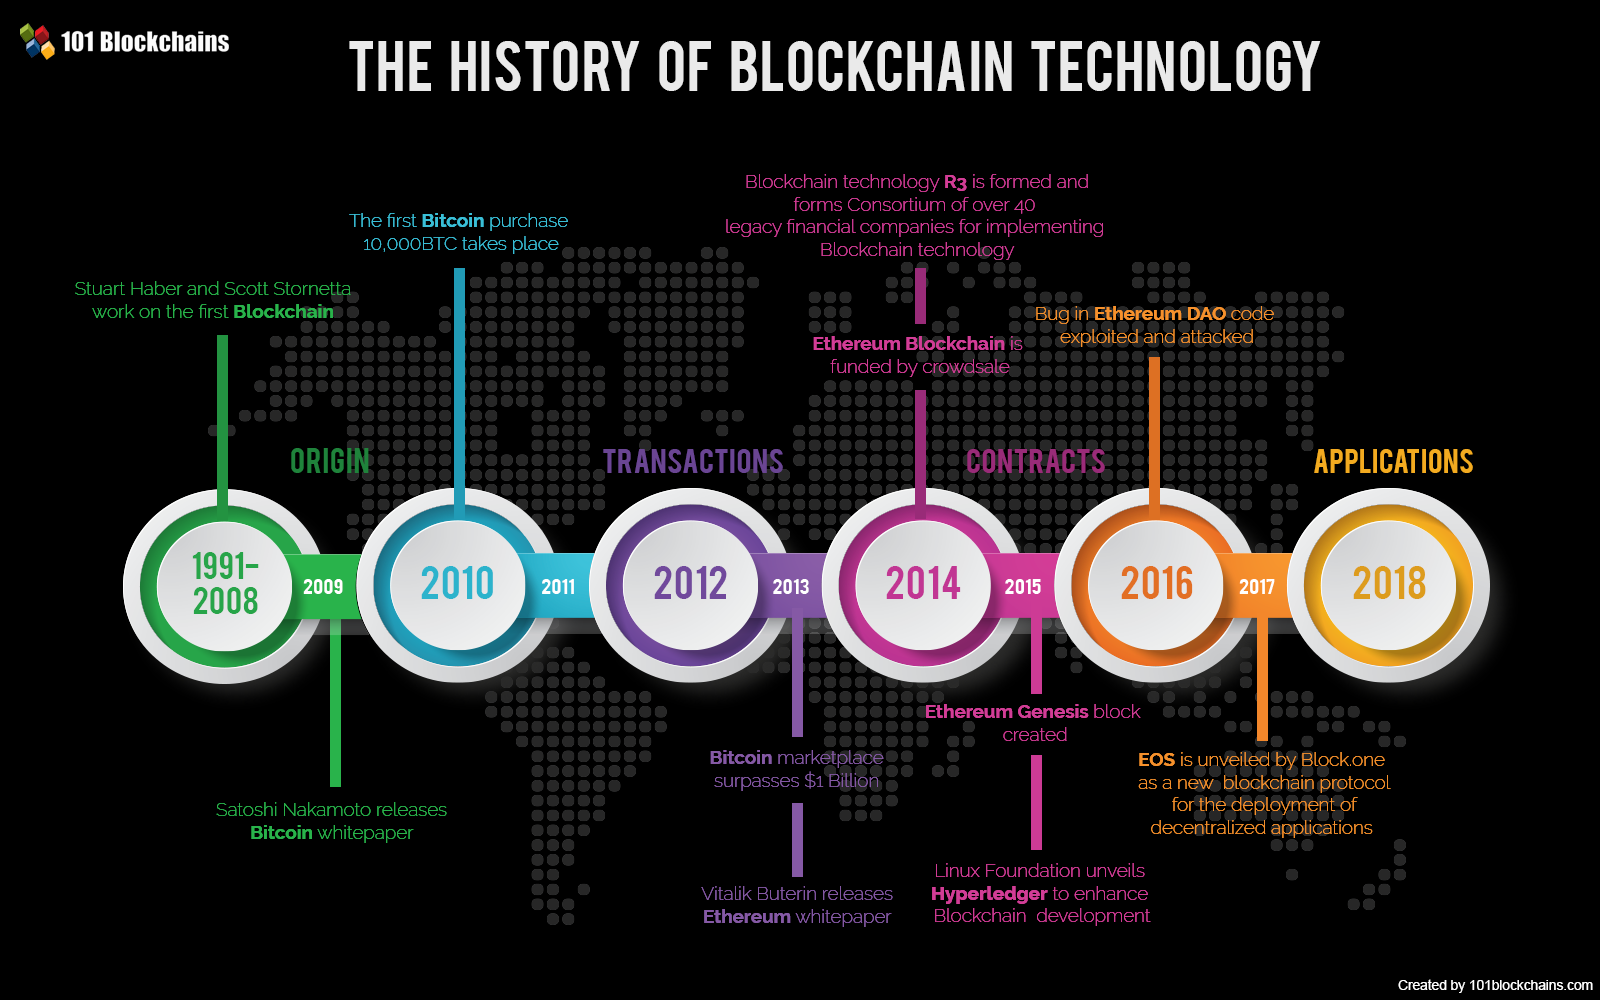
\includegraphics[width=0.8\linewidth]{History_of_Blockchain_Technology.png}
        \caption{Show the main steps of blockchain technology. \cite{HistoryBCT}}
        \label{fig:historyOfBlockchain}
    \end{figure}
    
    At the beginning there was the ledgers, a centralised system where everything were collected and stored, and obviously managed by only one organisation which becomes the 'custodian' and sole manager of the register. So, we have to trust this organisation to manage this records, for instance we have to trust banks to manage our bank accounts.
    
    Subsequently came the decentralised ledgers, which replicated the centralised structure in many smallest nodes. This improve the the degree of robustness and security, but within the field of the trust nothing changed, in fact this is managed by a unique organisation.
    
    Finally the distributed ledgers arrived. The distributed ledgers have eliminated the need for a central element responsible for the functioning and updating of the register.
    
    Blockchain is a specific category of Distributed Ledger Technologies.
    
    There are two fundamental concepts:
    \begin{itemize}
        \item[\textbf{Block}] It is a collection of transaction grouped in a unique block.
        \item[\textbf{Chain}] Each block is strongly connected to the previous one, the last block of the chain include the hash of the previous one. In this way if a block were modified it will broke the chain.
    \end{itemize}
    
    Main different kind of blockchain \cite{wiki-Blockchain, BlockchainPP}:
    \begin{itemize}
        \item \textbf{Public or Permissionless}: The network access is open to anyone and everyone, so it is completely free for everyone that would like to join. The control is distributed and involve every node. Everyone can join and everyone should validate the transaction.
        
        \item \textbf{Private or Permissioned}: The network access and the activity of control and validation are limited to a restricted group of members which follow some guide line (Governance of Blockchain). This kind of blockchain fits applications of companies or organisations that have to guarantee the authentication of participants and of nodes of the blockchain.
        
        
        \item \textbf{Consortium}: It is like the Private, but instead of a single organisation that manage the blockchain, there are more that perform this activity.
        
        \item \textbf{Hybrid}: The network access is limited to group of members that are recognised and authorised. The validation is entrusted to every nodes and all of them contribute to the network security.
    \end{itemize}
    \begin{figure}[h]
        \centering
        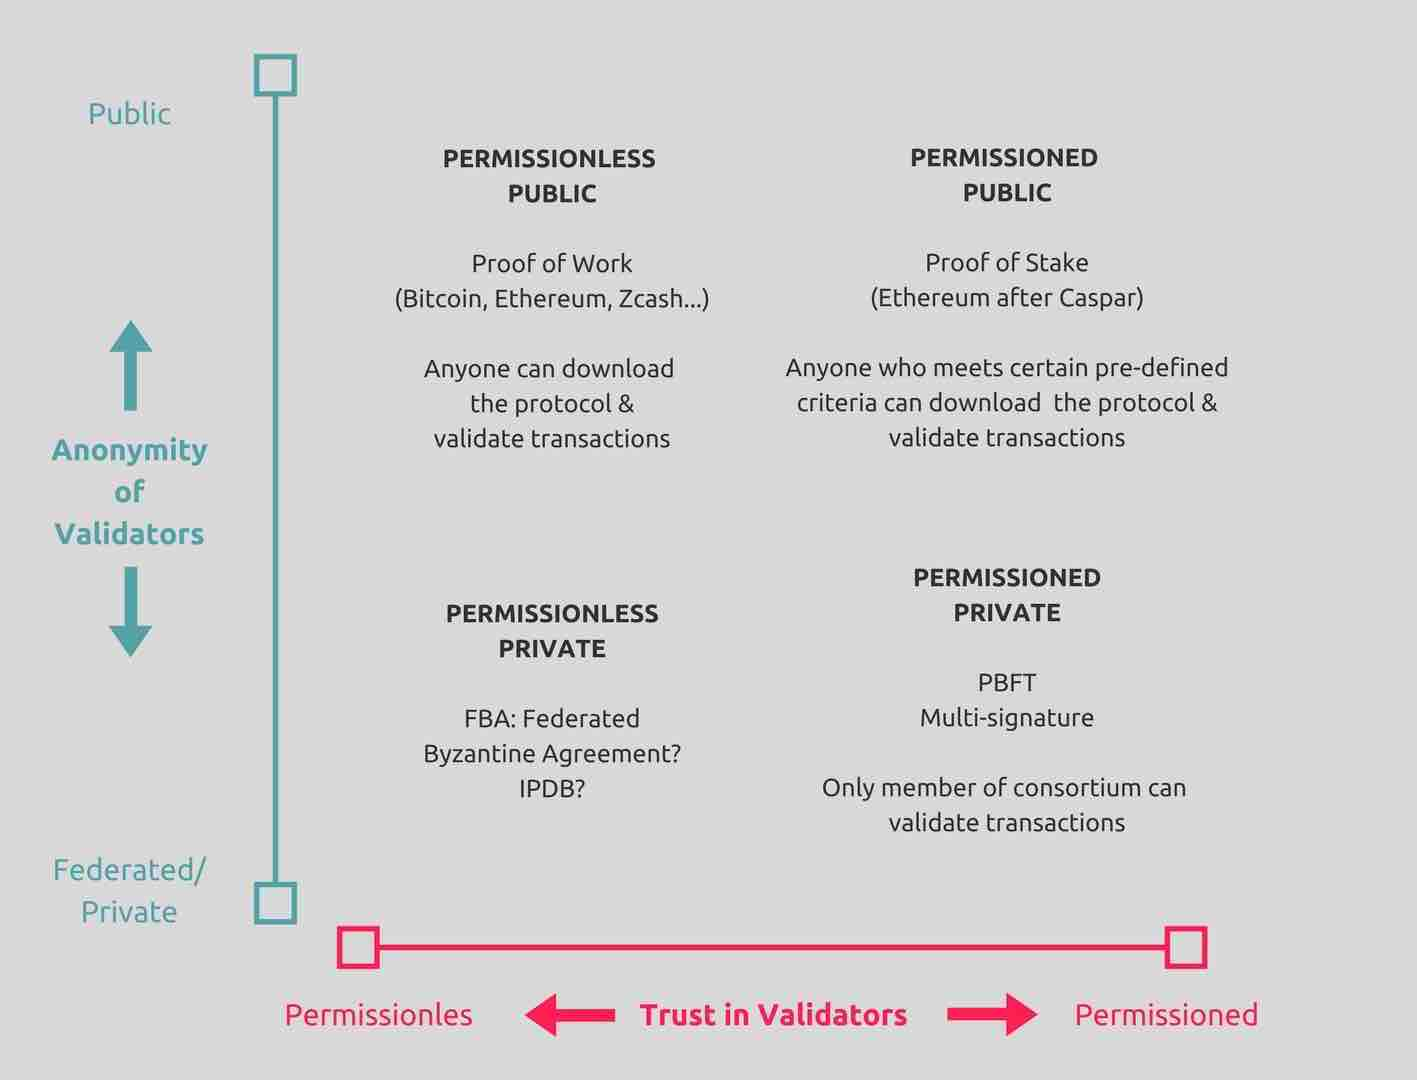
\includegraphics[width=0.8\linewidth]{pppp.jpg}
        \caption{This figure shows the possible combination of public, private and permissionless and permissioned. \cite{fig-pppp}}
        \label{fig:pppp}
    \end{figure}
    
\section{Blockchain as a Services}
    
    
\section{File Sharing}
    
   
    
    
    
\section{Governance OF the Internet vs Governance ON the Internet}
    
    
\section{Privacy vs Security}
   
    

\bibliographystyle{IEEEtran}  
\bibliography{references}

\end{document}
